\documentclass{beamer}
\usepackage{lmodern}
\usepackage{HECbeamer} 
% \usepackage{pgfpages}
% \pgfpagesuselayout{4 on 1}[letterpaper, landscape, border shrink=5mm]
\title[\color{white}{MATH60604A Collinearity}]{\texorpdfstring{MATH60604A \\Statistical modelling \\ \S 2h - Collinearity}{MATH60604A \\Statistical modelling \\ \S~2h - Collinearity}}
\author{Léo Belzile}
\institute{HEC Montréal\\
Department of Decision Sciences}
\date{} 
% \newcommand{\AIC}{\ensuremath{\mathsf{AIC}}}
% \newcommand{\BIC}{\ensuremath{\mathsf{BIC}}}
\begin{document}
\frame{\titlepage}

% \begin{frame}
% \frametitle{Examples of confounder}
% \bi 
% \item We could falsely think that coffee consumption has a significant effect on the appearance of a lung tumour; however, this effect disappears when adjusting for smoking status; smoker is a confounder for the effect of coffee because smokers tend to drink more coffee.
% \item The mortality rate in Florida is much higher than the rate in Michigan. This is mostly due to the fact Florida's population is much older on average than Michigan and older people are at a higher risk of death; age is a confounder for the effect of state.
% \item Potential remedies include 
% \bi \item \textbf{stratification} (compare mortality rates between Michigan and Florida separately for each age group), or 
% \item inclusion of the covariate in a regression model (along with other potential confounders).
% \ei
% \ei
% \end{frame}

\begin{frame}
\frametitle{Multicollinearity}
\bi
\item We say that two variables $\mathrm{X}_1$ and $\mathrm{X}_2$ are \alert{collinear} if
\bi
\vp
\item $\mathrm{X}_1$ and $\mathrm{X}_2$ are both correlated with $Y$
\item $\mathrm{X}_1$ and $\mathrm{X}_2$ are strongly correlated with each other --- so much so that they contain essentially the same information.
\ei
\item There could be multicollinearity between more than two variables\ldots in the same way that there could be more than one confounding variable.
\item In such a case, \alert{multicollinearity} (or simply collinearity) describes when an explanatory variable (or several) is strongly correlated with a linear combination of other explanatory variables.
\item One potential harm of multicollinearity is a \alert{decrease in precision} in parameter estimation, as it increases the standard errors of the parameters. 
\ei
\end{frame}

% 
% \begin{frame}
% \frametitle{Identifiability}
% \bi
% \item The variance inflation is due to the (near) lack of uniqueness of the least square solution (many combinations represent $Y$ equally well).
% \item The predicted or fitted values are unaffected.
% \item However, due to the (near) lack of identifiability, the estimated coefficients (and their standard errors) become numerically unstable.
% \ei 
% \end{frame}

\begin{frame}
\frametitle{A stupid illustration of multicollinearity}
\bi
\item Consider the log number of Bixi rentals per day as a function of the temperature in degrees Celcius and in Farenheit, rounded to the nearest unit. The postulated linear model is 
\begin{align*}
 \code{lognuser} = \beta_0 + \beta_{\code{c}} \code{celcius} + \beta_{\code{f}} \code{farenheit} + \varepsilon.
\end{align*}
\item The interpretation of $\beta_{\code{c}}$ is ``the average increase in number of rental per day when temperature increases by $1{}^{\circ}$C, keeping the temperature in Farenheit constant''\ldots
\item The two temperatures units are linearly related,
\[1.8 \code{celcius} + 32 = \code{farenheit}.\]
\ei
\end{frame}
\begin{frame}
\bi \item 
 Suppose that the true effect (fictional) effect of temperature on bike rental is 
 \begin{align*}
  \code{lognuser} = \alpha_0+ \alpha_1 \code{celcius} + \eps.
 \end{align*}
\item The coefficients for the model that only includes Farenheit are thus
 \begin{align*}
  \code{lognuser} = \gamma_0 + \gamma_1\code{farenheit} + \eps.
 \end{align*}
 where $\alpha_0 = \gamma_0 + 32\gamma_1$ and $1.8\gamma_1 = \alpha_1$.
 \item The parameters of the postulated linear model with both predictors, 
 \begin{align*}
 \code{lognuser} = \beta_0 + \beta_{\code{c}} \code{celcius} + \beta_{\code{f}} \code{farenheit} + \varepsilon,
\end{align*}
 are not \textbf{identifiable}, since any linear combination of the two solutions 
%  $k$, $\beta_0 = k\alpha_0 + (1-k)\gamma_0$, $\beta_1=k\alpha_1$ and $\beta_2=(1-k)\gamma_1$ 
gives the same answer.
\ei
\end{frame}

\begin{frame}[fragile]
 \frametitle{Bixi and multicollinearity}
 We consider a simple illustration with temperature at 16:00 in Celcius and Farenheit (rounded to the nearest unit for \code{rfarenheit}) to explain log of daily counts of Bixi users for 2014--2019. 
    \begin{figure}[ht!]
 \centering 
  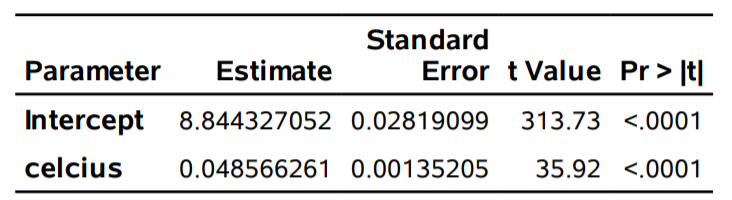
\includegraphics[width = 0.49\textwidth]{img/c2/slides3-e20} 
  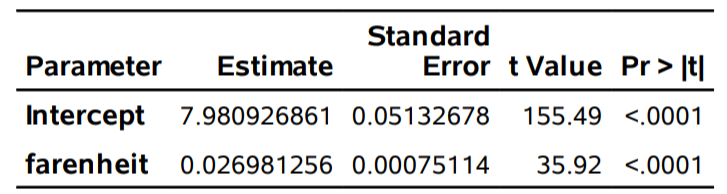
\includegraphics[width = 0.49\textwidth]{img/c2/slides3-e21}
 \end{figure}
 
   \begin{figure}[ht!]
 \centering 
  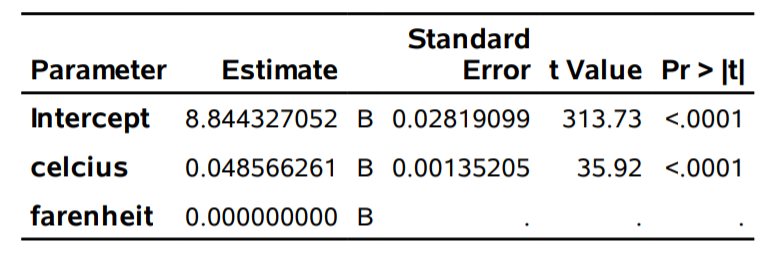
\includegraphics[width = 0.49\textwidth]{img/c2/slides3-e22} 
  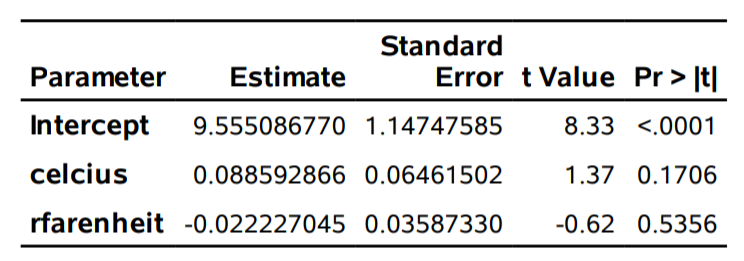
\includegraphics[width = 0.49\textwidth]{img/c2/slides3-e23}
 \end{figure}
 {\footnotesize \SASlang prints a warning if the data are exactly collinear.
 \begin{quote}
 \textbf{Note}: The X'X matrix has been found to be singular, and a generalized inverse was used to solve the normal equations. Terms whose estimates are followed by the letter 'B' are not uniquely estimable.
 \end{quote}
 
 }


\end{frame}

\begin{frame}{Effects of collinearity}
Generally, collinearity has the following effects:
\bi
\item The regression coefficients change drastically when new observations are included, or when we include/remove new covariates.
\item The standard errors of the coefficients in the multiple regression model are very high, since the $\bs{\beta}$ cannot be precisely estimated.
\item Consequently, the confidence intervals for these coefficients will be very wide.
\item The individual parameters are not statistically significant, but the global $F$-test indicates some covariates are nevertheless relevant.
\ei
\end{frame}


\begin{frame}[fragile]
\frametitle{How do we detect collinearity or confounders?}
\bi
\item If the variables are exactly collinear, \SASlang or \Rlang will drop redundant ones.
\bi 
\item The variables that are not \textbf{perfectly} collinear (e.g., due to rounding) will not be captured by software and will cause issues.
\ei
\item Look at the \textbf{linear correlation} between \alert{explanatory variables} and look at changes in estimated coefficients between regression models with and without a potential collinear variable.
\item The problem is that, when more than two variables are collinear, detection is hard.
\item One explanatory variable could be strongly correlated with a linear combination of other variables even though the individual correlations between the variables are not high. 
\ei
\end{frame}

\begin{frame}
\frametitle{Variance inflation factor}
\bi
\item Another tool we can use is the variance inflation factor ($\mathsf{VIF}$); in \SASlang, use the option \code{vif} inside \code{proc reg}.
\item For a given explanatory variable $\mathrm{X}_j$, its $\mathsf{VIF}$ is
\begin{align*}
\mathsf{VIF}(j)=\frac{1}{1-R^2(j)}
\end{align*}
where $R^2(j)$ is the $R^2$ of the model obtained by regressing $\mathrm{X}_j$ on all the other explanatory variables.
 \item The tolerance factor, $\mathsf{TOL}=1-R^2(j)$, is the reciprocal of $\code{VIF}$.
\ei
\end{frame}
\begin{frame}
\frametitle{When is collinearity an issue?}
\bi
\item $R^2(j)$ represents the proportion of the variance of $\mathrm{X}_j$ that is explained by all the other predictor variables.
\item When is collinearity problematic? There is no general agreement, but practitioners typically choose an arbitrary cutoff (rule of thumb)
\bi 
\item $\mathsf{VIF}(j) > 4$ or $\mathsf{TOL} < 0.25$ implies that $R^2(j) >0.75$
\item $\mathsf{VIF}(j) > 5$ or $\mathsf{TOL} < 0.2$ implies that $R^2(j) >0.8$
\item $\mathsf{VIF}(j) > 10$ or $\mathsf{TOL} < 0.1$  implies that $R^2(j) >0.9$
\ei
\ei
\end{frame}






\begin{frame}
 \frametitle{Observations for Bixi multicollinearity example}
 \bi 
 \item The value of the $F$ statistic for the global significance for the simple linear model with Celcius (not reported) is $1292$ with associated $p$-value less than $0.0001$, suggesting that temperature is statistically significant ($5$\% increase in number of users for each increase of $1^{\circ}$C).
 \item Yet, when we include both Celcius and Farenheit (rounded), the individual coefficients are not significant anymore at the 5\% level.
 \item Moreover, the sign of \code{rfarenheit} change relative to that of \code{farenheit}!
  \item Note that the standard errors for Celcius are $48$ times bigger when including the two covariates.
 \item The variance inflation factors of both \code{rfarenheit} and \code{celcius} are enormous ($2454.68$), suggesting identifiability issues. 
\ei
\end{frame}
\begin{frame}[fragile]
 \frametitle{Added-variable plots for Bixi multicollinearity example}
 
 \begin{figure}
  \centering 
  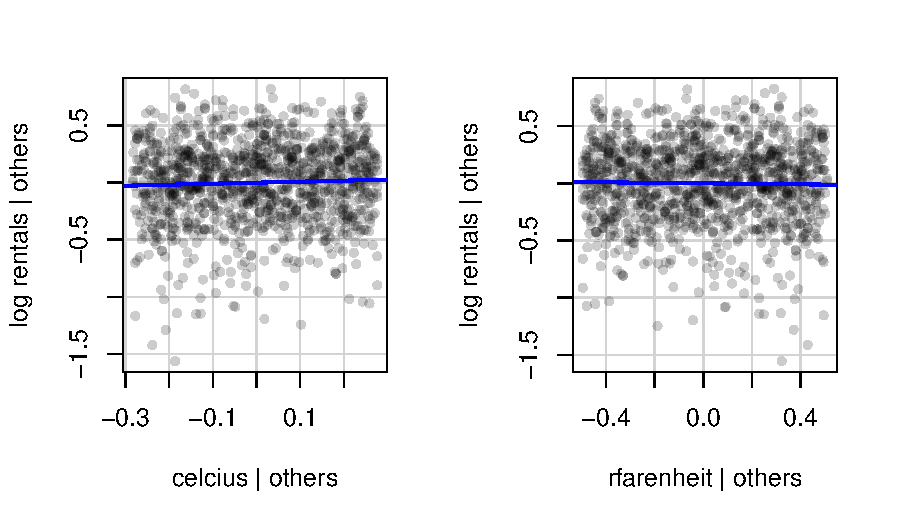
\includegraphics[width = \textwidth]{img/c2/03-linreg-avplot_temp.pdf}
 \end{figure}

\end{frame}




\begin{frame}
\frametitle{Fictional example of multicollinearity}
\bi
\item We consider a fictional example with 100 observations on the outcome variable
$Y$ as well as five predictor variables $\mathrm{X}_1$ through $\mathrm{X}_5$. 

\item  The $Y$ values were actually randomly generated under the following model
\begin{align*}
Y=\mathrm{X}_1+\mathrm{X}_2+\mathrm{X}_3+\mathrm{X}_4+\mathrm{X}_5+\varepsilon
\end{align*}
\item The parameter associated with each variable is $1$.
\item The data can be found in \code{simcollinear.sas7bdat}.
\ei
\end{frame}

\begin{frame}[fragile]
\frametitle{Fictional example of multicollinearity}
\bi
\item The correlation matrix between all the variables
\vp \vp
\begin{tcolorbox}[colback=white,colframe=hecblue,title=\SASlang code for correlation]
\begin{verbatim}
proc corr data=statmod.simcollinear noprob;
var y x1-x5;
run;
\end{verbatim}
\end{tcolorbox}
\begin{center}
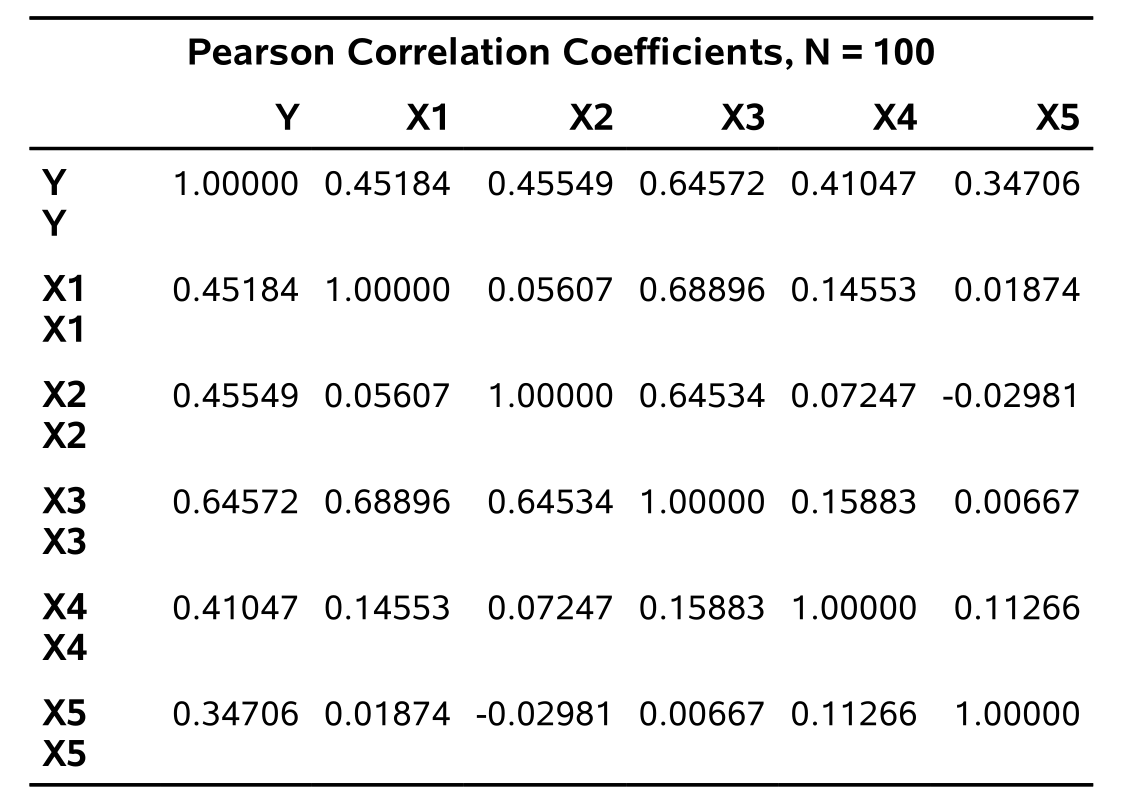
\includegraphics[width= 0.6\linewidth]{img/c2/slides3-e24}
\end{center}
\ei
\end{frame}

\begin{frame}[fragile]
\frametitle{Simple regression for the fictional example of multicollinearity}
\bi
\item The correlation between $Y$ and each predictor variable is significant and positive. 
\item Consequently, if we fit a separate model for each predictor variable, the parameter for each variable would be significant and positive for each one. This is consistent with the true model from which we simulated the data. 
\item This shows that there are enough observations to estimate the parameters, and to make proper conclusions about their effects, at least when considering one predictor at a time.
\ei
\end{frame}

\begin{frame}[fragile]
\frametitle{Fictional example of multicollinearity}
\bi
\item However, $\mathrm{X}_1$, $\mathrm{X}_2$ et $\mathrm{X}_3$ are highly correlated with each other which could cause multicollinearity problems.
\item We fit the model containing all the predictor variables with \code{proc reg}, while requesting multicollinearity diagnostics. 
\vp \vp
\begin{tcolorbox}[colback=white,colframe=hecblue,title=\SASlang code to compute variance inflation factor]
\begin{verbatim}
proc reg data=statmod.simcollinear; 
model y=x1-x5 / vif; 
run;

proc glm data=statmod.simcollinear;
model y=x1-x5 / ss3 solution tolerance;
run;
\end{verbatim}
\end{tcolorbox}
\ei
\end{frame}
\begin{frame}{\SASlang procedures: \code{reg} versus \code{glm}}
The \code{glm} procedure doesn't include an option to compute the \code{vif}; one can either use \code{tol} (reciprocal of $\mathsf{VIF}$) or else resort to the \code{reg} procedure for fitting linear models. 
\bi \item By default, diagnostic plots are produced by \code{reg} (\code{plots=diagnostics} option with \code{glm}).
\item The \code{reg} procedure includes more model selection diagnostics (not used in inference).
\item The table of coefficients is automatically printed by \code{reg} (\code{solution} option in \code{glm}).
\item The main drawback of \code{reg} is that it doesn't handle categorical variables: these must be manually coded using binary indicators (\code{0}-\code{1})  (\textbf{frequent programming mistake}).
\ei
 
\end{frame}


 \begin{frame}
\frametitle{Parameter estimates and VIF}
\begin{center}
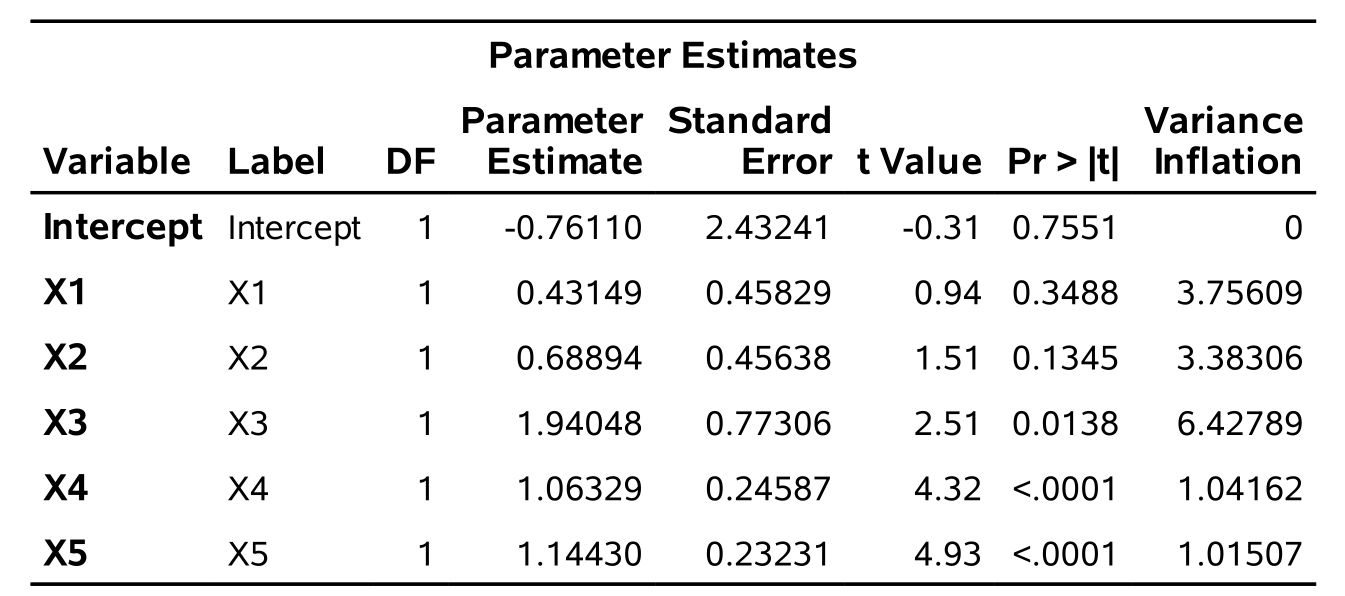
\includegraphics[width= 0.8\linewidth]{img/c2/slides3-e25}
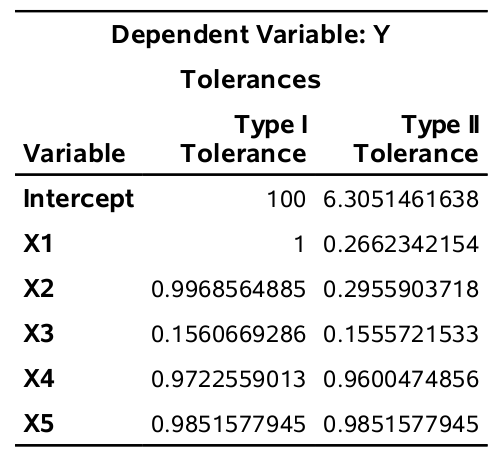
\includegraphics[width= 0.4\linewidth]{img/c2/slides3-e26}
\end{center}
\end{frame}

\begin{frame}[fragile]
\frametitle{Goodness of fit and model summary}
\bi
\item Overall, the model seems adequate. The $R^2$ is $62\%$. 
\item However, the variables $\mathrm{X}_1$ and $\mathrm{X}_2$ are no longer significant once other explanatories are accounted for.
\item The $\mathsf{VIF}$ of $\mathrm{X}_3$ is quite large ($6.43$) and the variance inflation factors for $\mathrm{X}_1$ and $\mathrm{X}_2$ are between $3$ and $4$.
\item \textbf{This indicates a possible problem of collinearity}. The estimation precision for these parameters is not as good as it would be if there were no multicollinearity. 
\item Note that the $\mathsf{VIF}$ is an individual measure. It does not tell us which particular variables are correlated with each other.
\ei
\end{frame}


\end{document}
